\chapter{Implementation and Evaluation}
\label{chap:eval}
\section{Imlementation}
The portable probabilistic programming framework is implemented in C and included four parts: parse, infer, query and API implementations.

\subsection{Parser}
We implemented the parser based on the grammar in Chapter ~\ref{chap:approach} Section ~\ref{sec:syntax}. Since the language is used to describe Bayesian networks, we didn't generate abstract syntax tree. Instead, we generate the graph to describe the probabilistic graphical model with the following data structure:
\begin{lstlisting}[language=C]
  struct BNVertex {
    int type;      // draw or compute
    float sample;  // last sampled value
  };
 
  struct BNVertexDraw {
    struct BNVertex super;  // extends BNVertex
    int type;               // dbern, dnorm, dgamma, or constant
  };
 
  struct BNVertexDrawBern {
    struct BNVertexDraw super;
    float p;
  };
 
  struct BNVertexDrawNorm {
    struct BNVertexDraw super;
    float mean;
    float variance;
  };
 
  struct BNVertexDrawGamma {
    struct BNVertexDraw super;
    float a;
    float b;
  };
 
  struct BNVertexDrawConst {
    struct BNVertexDraw super;
    float c;
  };
 
  struct BNVertexCompute {
    struct BNVertex super;  // extends BNVertex
    int type;               // + or if
  };
 
  struct BNVertexComputePlus {
    struct BNVertexCompute super;
    struct BNVertex* left;
    struct BNVertex* right;
  };
 
  struct BNVertexComputeIf {
    struct BNVertexCompute super;
    struct BNVertex* condition;
    struct BNVertex* consequent;
    struct BNVertex* alternative;
  };
\end{lstlisting}
The generated network is (1) constructed, (2) topological sorted, and (3) stored in an array struct \texttt{BNVertex* vertices[]}. The inference engine can traverse this array from the start to the end, and access sample values stored in the vertices. Because the network is already topological sorted, it is guaranteed that inference engine always reads the correct sample values.

Users can declare many probabilistic graphical models in our declarative programming language. Figure ~\ref{fig:hmm} shows an example of Hidden Markov Model(HMM) described in our language and Figure ~\ref{fig:ldacode} shows an example of Latent Dirichlet Allocation(LDA).

\begin{figure}
  \begin{lstlisting}[language=C]
    model hidden_markov_model(n, a, b) {
        // n -- chain length
        // a -- number of possible states
        // b -- number of possible observations
        public states[n]   // hidden states
        public observ[n]   // observations
        public trans[a,a]  // transition matrix of size a*a
        public emiss[a,b]  // emission matrix of size a*b
        public start[a]    // start probabilities of size a

        states[0] ~ dcat(start)
        for i = 1 to n-1 {
            states[i] ~ dcat(trans[states[i-1]])
        }

        for i = 0 to n-1 {
            observ[i] ~ dcat(emiss[states[i]])
        }
    }
  \end{lstlisting}
  \caption{An HMM example}
  \label{fig:hmm}
\end{figure}

\begin{figure}
  \begin{lstlisting}[language=C]
    model latent_dirichlet_allocation(k, num_docs, num_words[], vocab_size) {
      for i = 1 to k {
        topics(i, :) = dirichlet(1, vocab_size);
      }
      
      for i = 1 to num_docs {
        topic_dist = dirichlet(1, k);
        for j = 1 to num_words(i) {
          topic = multinomial(topic_dist);
          X{i}(j) = multinomial(topics(topic, :));
        }
      }
    }
  \end{lstlisting}
  \caption{An LDA example}
  \label{fig:lda}
\end{figure}
\subsection{Probabilistic Distributions}
The implementations of the probabilistic distributions are generally based on rejection sampling. We leveraged the algorithms in probability theory to generate variables from a specified distribution.

Figure ~\ref{fig:gaussian} is an example to show how we derive the samples of Gaussian distribution from randomC distribution which generate random values in $[0, 1]$:

\begin{figure}
\begin{lstlisting}[language=C]
  float gaussian(float mu, float sigma)
  {
      float u, v, x, y, q;
      do {
          u = 1 - randomC();
          v = 1.7156 * (randomC() - 0.5
          x = u - 0.449871;
          y = fabs(v) + 0.386595;
          q = x * x + y * (0.196 * y - 0.25472 * x);
      } while (q >= 0.27597 && (q > 0.27846 || v * v > -4 * u * u * log(u)));
      return mu + sigma * v / u;
  }
\end{lstlisting}
\caption{Sampling Gaussian distribution}
\label{fig:gaussian}
\end{figure}

\subsection{Inference Engine}

\begin{figure}
    \centering
    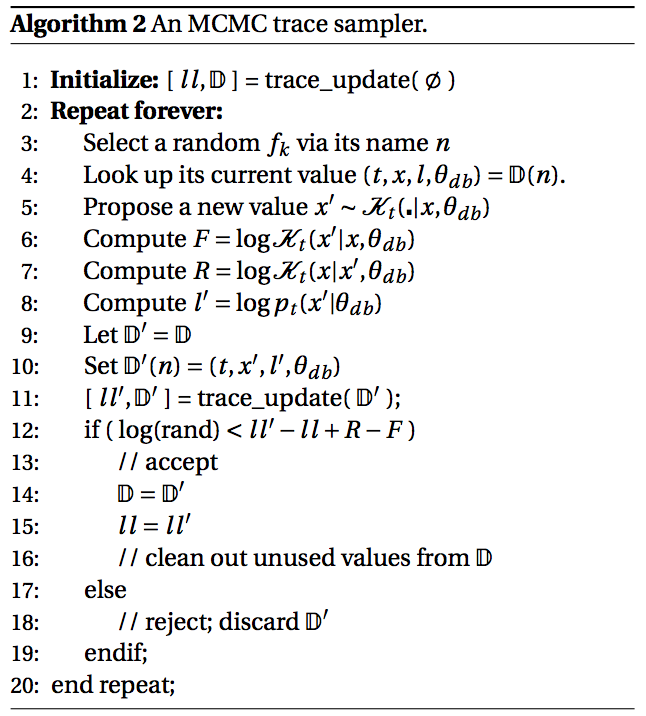
\includegraphics[width=0.7\textwidth]{figures/trace1.png}
    \caption{An MCMC trace sampler.}
    \label{fig:trace1}
\end{figure}

\begin{figure}
    \centering
    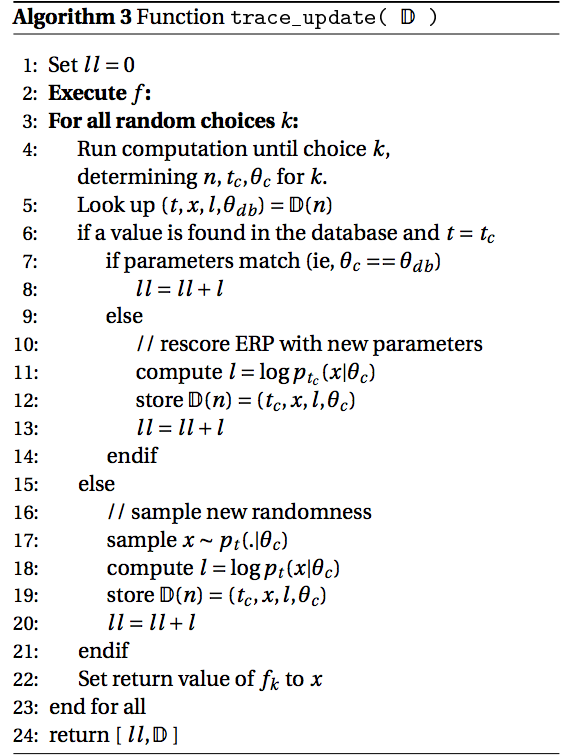
\includegraphics[width=0.7\textwidth]{figures/trace2.png}
    \caption{Algorithm for trace update}
    \label{fig:trace2}
\end{figure}

In the implementation of the MH alorithm in our inference engine, we leverage the approach proposed by ~\cite{lightweight}, which memorized trace information and update trace iteratively as illustrated in Figure ~\ref{fig:trace1} and Figure ~\ref{fig:trace2}. 

There are some other methods to implement an inference engine such as \cite{nonstandard}, which showed how \textit{nonstandard interpretations} of probabilistic programs can be used to perform efficient inference algorithms. In their method, infromation about the structure of the distributions (which is the dependencies or gradients in the probabilistic graphical models) is derived as monad-like side computation as the same time of executing the program. Meanwhile, the interpreations can be coded easily with some special-purpose objects and operator overloading. They promoted the inference efficiency perfomance by using the structure information of distribution as part of the variety of infreence algorithms.

Additionally, because of the program is in a machine-readable form, various of techniques from compiler design and program analysis can be used in the inference engine. ~\cite{gordon2013} designed a new model-learner pattern for Bayesian reasoning. In their work, a new probabilistic programming abstraction was proposed, a typed Bayesian model, based on a pair of probabilistic expressions for the prior and sampling distributions. Also, ~\cite{dataflow} presented a new algorithm for Bayesian inference over probabilistic programs, whihc is based on data flow analysis techniques from the program analysis community.

\subsection{API}
To enable the APIs for other programming languages, we first compiled the inferface file as showed in Section ~\ref{sec:api} and generated the wrapper code that other languages need to access the underlying C/C++ code. Then the users will have access to the APIs of the portable probabilistic programming language framework in their domain language. 

\section{Experiments}
\begin{figure}
    \centering
    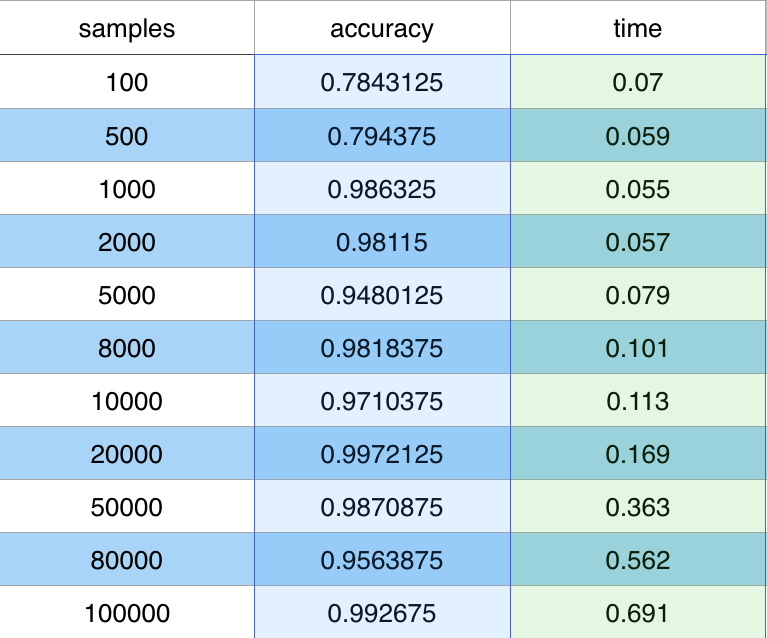
\includegraphics[width=0.7\textwidth]{figures/flip_eval1.png}
    \caption{Table of flip example}
    \label{fig:flip_eval1}
\end{figure}

\begin{figure}
    \centering
    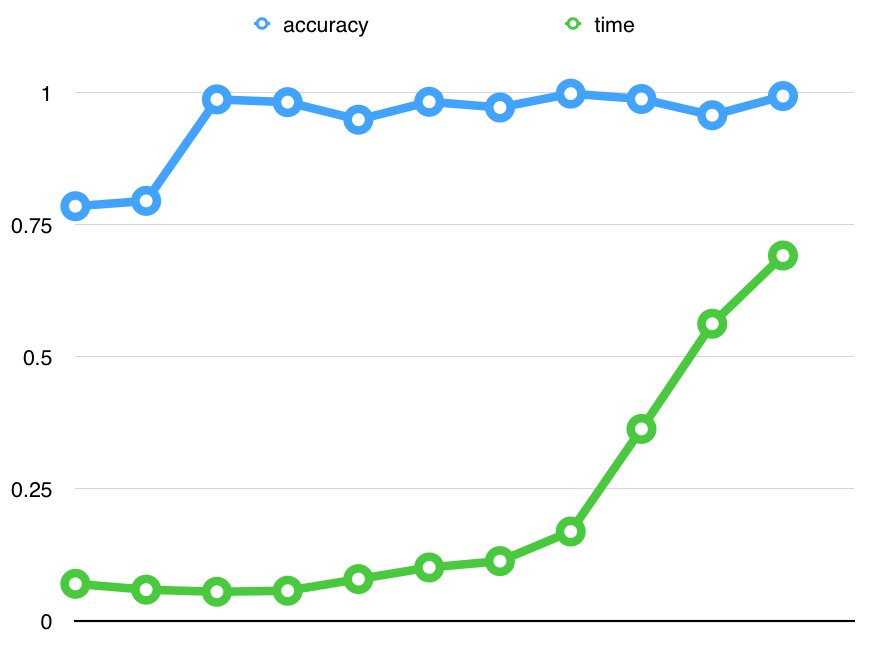
\includegraphics[width=0.7\textwidth]{figures/flip_eval2.png}
    \caption{Evaluation of accuracy and time according to the number of samples.}
    \label{fig:flip_eval2}
\end{figure}
We have evaluated several examples in the framework. 
For the flip example as is showed in ~\ref{fig:flip_eg}, the benchmark is showed in Figure ~\ref{fig:flip_eval1} and Figure ~\ref{fig:flip_eval2}.
